\section{Introduzione}

	\subsection{Il Gioco}
		Il gioco implementato per questo progetto si ispira e ne imita le meccaniche del famoso  Flappy Bird. L'obiettivo del giocatore mantenere in volo il proprio personaggio, nel nostro caso una palla di fuoco, e far sì che non collida con gli altri elementi del gioco. Il giocatore interagisce solo dando una spinta verso l'alto attraverso il semplice tap su schermo. Oltre a questo per guadagnare punti deve attraversare un piccolo spazio tra una coppia di stalattiti a cui il personaggio va incontro.
		
		Abbiamo scelto questa gioco perché nella sua semplicità è un ottimo progetto didattico per provare e imparare ad usare un framework cross-platform.
			
		\subsubsection{Elementi di gioco}
			Il gioco è costituito dai seguenti elementi:
			\begin{itemize}
				\item Il giocatore: \textbf{una palla di fuoco} soggetta alla fisica, l'utente interagisce con essa applicando una forza verso l'alto con un semplice tap sullo schermo;
				\item \textbf{Coppie di stalattiti} a distanza costante e con uno spazio fra esse casuale. Il giocatore dovrà passarci attraverso per guadagnare punti se collide con essi invece il gioco termina.
				\item \textbf{Terreno e limite del cielo}: se la palla di fuoco collide con essi il gioco termina;
				\item Uno \textbf{sfondo scorrevole}.
			\end{itemize}
		
		\subsubsection{Schermate}
			Le schermate sono:
			\begin{itemize}
				\item Menu principale;
				\item Gioco;
				\item Game over;
				\item Menu di gioco: corrisponde al menu principale ma si sovrappone alla scena di gioco.
			\end{itemize}
		
		\subsubsection{Menu}
			Il gioco deve presentare il menu con le seguenti voci:
			\begin{itemize}
				\item Play/Resume/Restart: la label cambia in base allo stato del gioco;
				\item Options:
				\begin{itemize}
					\item Volume: modifica il volume dell'audio dell'applicazione;
					\item Costume: consente all'utente di cambiare stile della propria palla di fuoco;
				\end{itemize}
				\item Best score: per visualizzare il miglior punteggio fatto;
				\item Info: una schermata dove in poche righe viene spiegato il gioco.
			\end{itemize}
		
		\subsubsection{Sonoro}
			Per il sonoro sono state utilizzate 3 musiche la cui riproduzione parte a seguito dei seguenti eventi:
			\begin{itemize}
				\item Apertura del menu di gioco\ref{fig:menu};
				\item Gioco avviato\ref{fig:game};
				\item Game Over.
			\end{itemize}
	

	
	\subsection{Sviluppo: i frameworks}
		Oggigiorno esistono numerosi framework per sviluppare videogame mobile multipiattaforma. \textbf{Unity3D} e \textbf{Corona SDK} sono due di questi e sono stati scelti per sperimentarne le differenze nel processo di sviluppo di Flappy Flame.
		
		\subsubsection{Unity3D}
			Unity è un framework, ovvero uno strumento di authoring integrato multipiattaforma utilizzato per la creazione di videogiochi 3D o di altri contenuti interattivi. 
			L'ambiente di sviluppo Unity gira sia su Microsoft Windows sia su macOS e i giochi che produce possono essere eseguiti su varie piattaforme, come Linux, Xbox 360, PlayStation 3, iPad, iPhone e Android. 
			Unity permette poi di utilizzare sia un editor per lo sviluppo e la progettazione di contenuti sia un motore di gioco per l'esecuzione del prodotto finale. 
			Dunque, le caratteristiche principali di Unity sono:
			\begin{enumerate}
				\item Integrated development environment con la gerarchia degli oggetti, editor visuale, un dettagliato visualizzatore delle proprietà e un'anteprima dal vivo del gioco;
				\item Sviluppo su molte piattaforme;
				\item Molti file possono essere caricati in Unity e vengono importati automaticamente. Se subiscono modifiche vengono ri-esportati automaticamente.
			\end{enumerate}
		
		\subsubsection{Corona SDK}
			Corona SDK è un framework cross-platform per lo sviluppo di app, in particolare offre delle API per un motore grafico 2D, essenziale per minimizzare lo sviluppo di videogame. Il framework si appoggia al linguaggio di scripting Lua: linguaggio molto famoso nel mondo degli sviluppatori di videogame data la sua alta efficienza e facilità di utilizzo. Il framework può essere esteso grazie a Plugin e permette di interfacciarsi alle API native delle maggiori piattaforme qualora ci sia la necessità. Inoltre è completamente gratuito (è richiesta solo la registrazione) e i software da esso prodotti possono essere commercializzati senza nessun costo aggiuntivo.
		
		
	\subsection{Struttura del documento}
		La presente sezione è stata scritta da entrambi gli autori. Le sezioni che coinvolgono la discussione dello sviluppo con lo specifico framework sono scritte dall'autore segnalato sotto al titolo della sezione. Le sezioni \ref{sec:unity} e \ref{sec:corona} sono indipendenti tra loro e data la notevole differenza dei due framework non seguono la stessa struttura. Nell'ultima sezione invece si metteranno a confronto il processo e i risultati ottenuti dall'utilizzo di questi framework.
		
	\newpage
	\begin{figure} [h!]
		\centering
		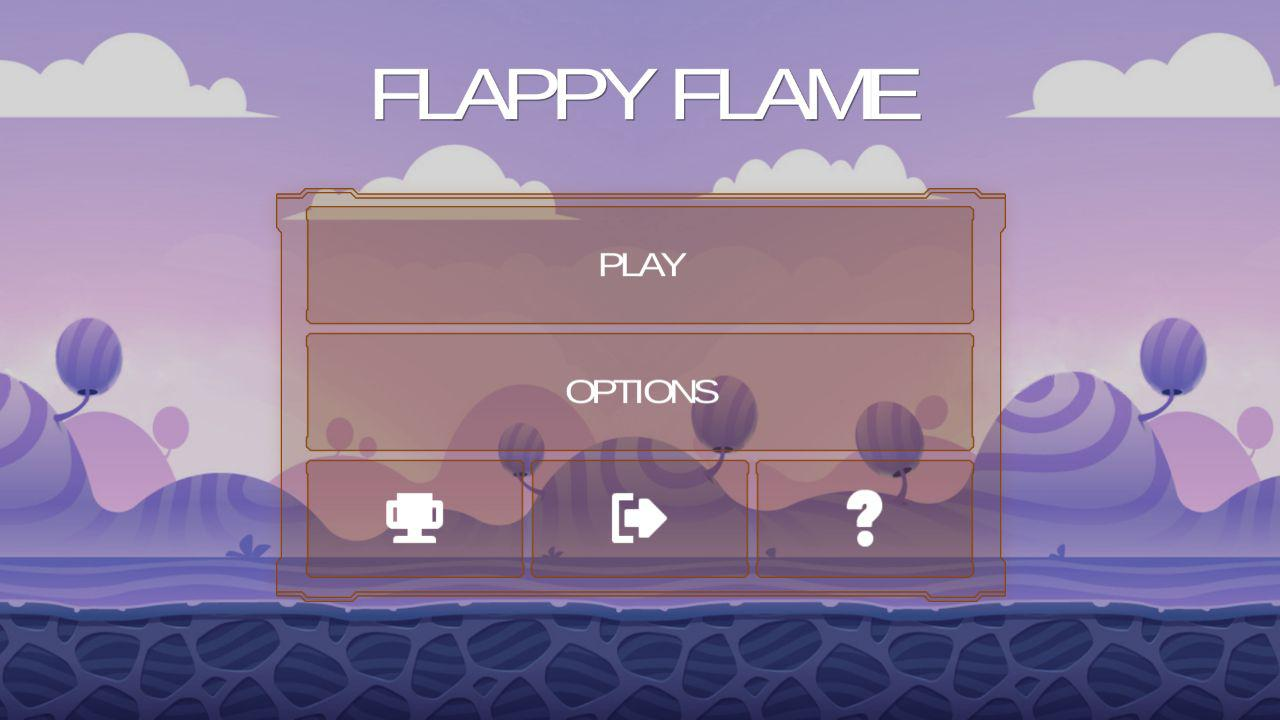
\includegraphics[width=\textwidth]{img/unityMenu}
		
		\vspace{2cm}
		
		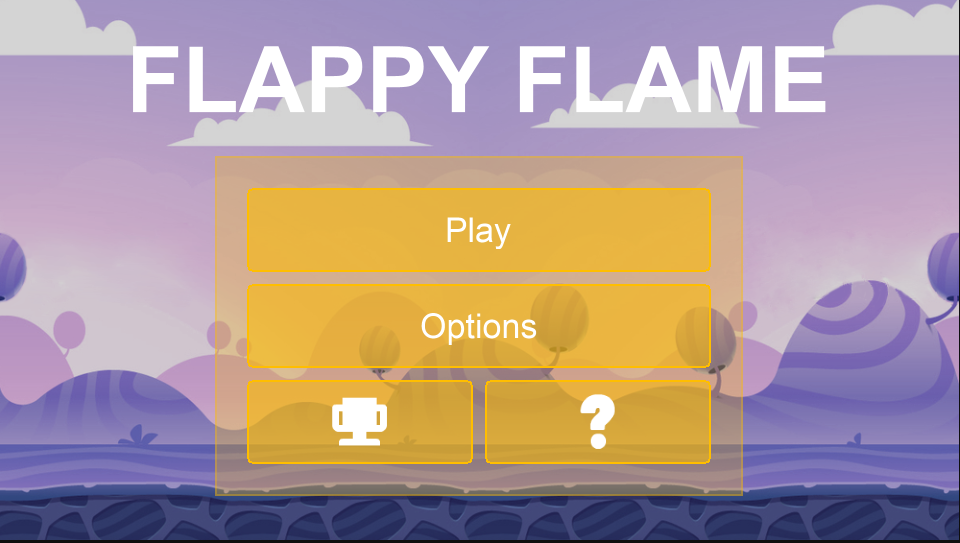
\includegraphics[width=\textwidth]{img/coronaMenu}
		\caption{Menu principale in Unity3D (in alto) e Corona SDK}
		\label{fig:menu}
	\end{figure}
	
	\newpage
	\begin{figure} [h!]
		\centering
		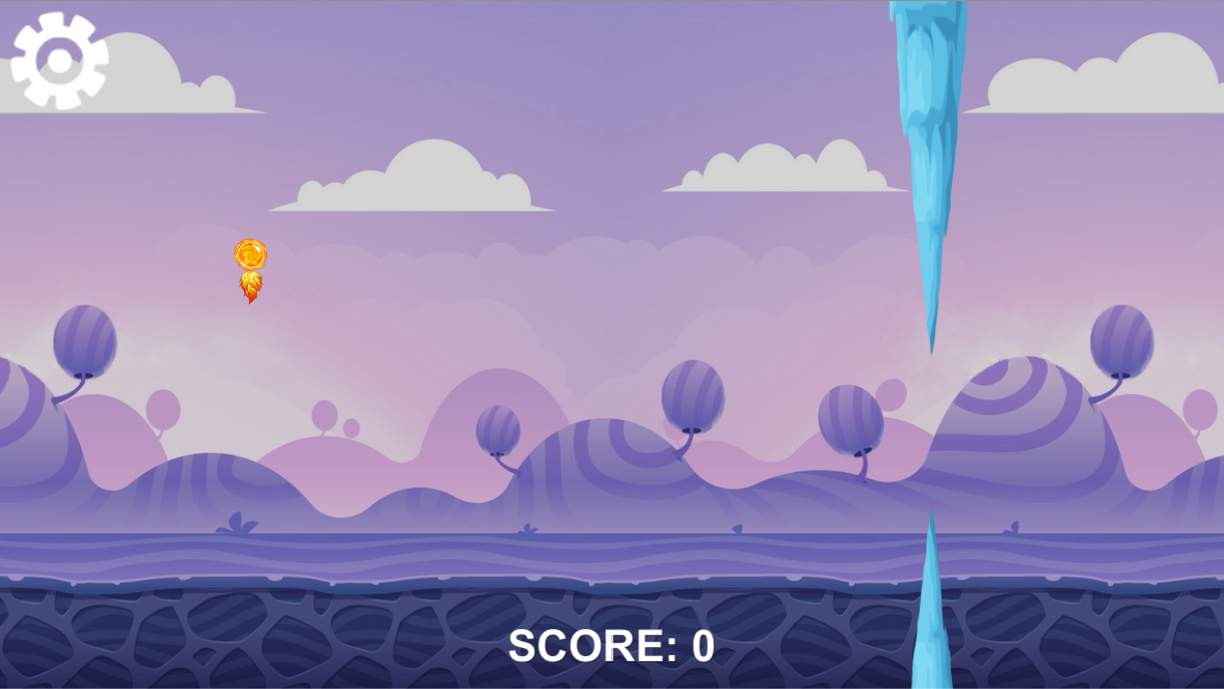
\includegraphics[width=\textwidth]{img/unityGame}
		
		\vspace{2cm}
		
		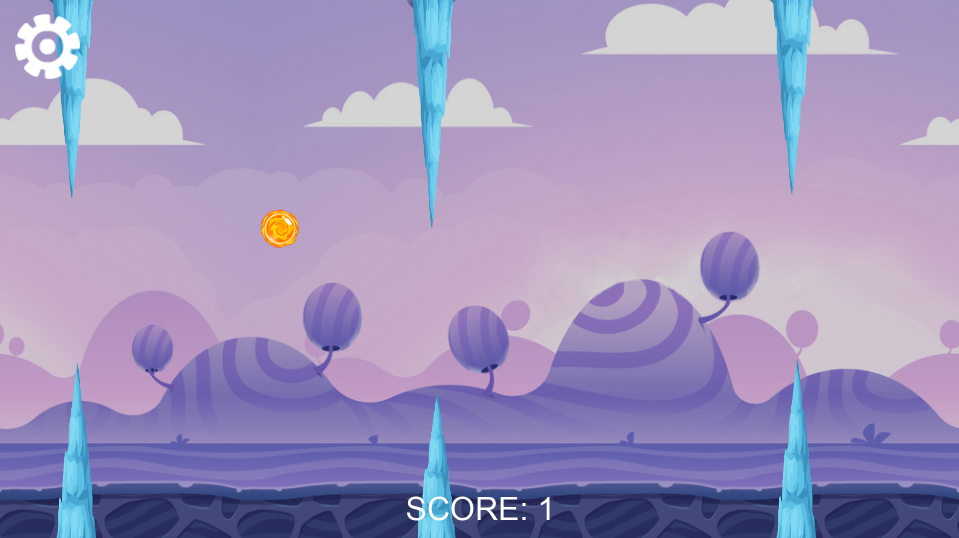
\includegraphics[width=\textwidth]{img/coronaGame}
		\caption{Schermata di gioco in Unity3D (in alto) e Corona SDK}
		\label{fig:game}
	\end{figure}
	
	\newpage
	
	